% !TEX root = ../main.tex
\section{Поняття випадкового вектора}
В багатьох прикладних задачах розглядають не одну випадкову величину,
а деяку їх систему. Наприклад,
стан деякого приладу характеризується станом його компонентів,
які в кожен момент можуть вийти з ладу, причому відмова одного компоненту 
може пришвидшити відмову інших.
Системою випадкових величин також можна описати оцінки
навмання вибраного випускника університету, і в цьому випадку теж
можуть виникати деякі залежності між оцінками з різних дисциплін.
Ці приклади показують, що дослідження
систем випадкових величин є складнішим за дослідження окремих величин,
тому що необхідно враховувати, як ці величини можуть бути пов'язані між собою.

\begin{definition}\index{випадковий вектор}
    Нехай $\left\{\Omega, \mathcal{F}, \P \right\}$ --- ймовірнісний просторі
    деякого стохастичного експерименту.
    \emph{Випадковим вектором (системою випадкових величин)}
    називається вимірна функція $\vec{\xi}(\omega) = 
    \left(\xi_1(\omega), \xi_2(\omega), ... , \xi_n(\omega)\right)^{T}: \Omega \rightarrow \mathbb{R}^n$, де
    під вимірністю мається на увазі, що 
    \begin{equation*}
        \forall \vec{x} \in \mathbb{R}^n: 
        A=\left\{\omega \in \Omega: \xi_1(\omega) < x_1, 
                                    \xi_2(\omega) < x_2,
                                    ... ,
                                    \xi_n(\omega) < x_n\right\}
        \in \mathcal{F}
    \end{equation*}
\end{definition}
\begin{remark}
    Можна довести інтуїтивно зрозумілий факт: координати випадкового вектора є випадковими величинами в сенсі означення 
    \ref{def:random_variable}, і навпаки --- функція з $\Omega$ в $\mathbb{R}^n$, координатами якої є випадкові величини,
    є випадковим вектором в сенсі наведеного вище означення.
\end{remark}
Випадковий вектор можна трактувати як випадкову точку в $\mathbb{R}^n$.
Наприклад, при $n = 2$ $\vec{\xi} = (\xi_1, \xi_2)^T$ --- випадкова точка на площині. 

\subsection{Сумісна функція розподілу}
Як у і випадку випадкових величин, випадковий вектор теж характеризується своєю функцією розподілу.
Спочатку розглянемо лише двовимірний випадок, оскільки його простіше інтерпретувати геометрично.
\begin{definition} \index{функція розподілу!сумісна}
    \emph{Сумісною функцією розподілу} двовимірного випадкового вектора $\vec{\xi}$ 
    називається $F_{\vec{\xi}}(x, y) = \P\left\{\omega: \xi_1 < x, \xi_2 < y\right\}$, $x, y \in \mathbb{R}$.
\end{definition}
Значення $F_{\vec{\xi}}(x, y)$ рівне ймовірності 
    потрапляння точки в нескінченний квадрант з вершиною в точці $(x, y)$.
\begin{center}
    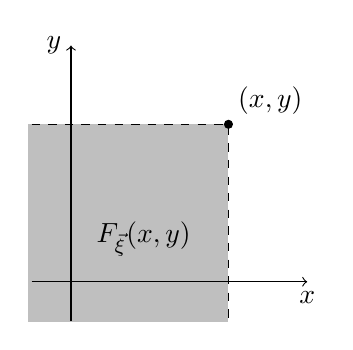
\begin{tikzpicture}[baseline={(current bounding box.north)}]
        \fill [lightgray] (2, 2) rectangle (-0.55, -0.51);
        \draw [->] (-0.5, 0) -- (3, 0);
        \draw [->] (0, -0.5) -- (0, 3);
        \draw [fill] (2, 2) circle [radius=0.05];
        \node [above right] at (2, 2) {$(x, y)$};
        \draw [dashed] (-0.5, 2) -- (2, 2) -- (2, -0.5);
        \node [below] at (3, 0) {$x$};
        \node [above right] at (0.2, 0.2) {$F_{\vec{\xi}}(x, y)$};
        \node [left] at (0, 3) {$y$};
    \end{tikzpicture}
\end{center}

\noindent\textbf{Властивості сумісної функції розподілу:}
\begin{enumerate}
    \item Область визначення --- $\mathbb{R}^2$, область значень --- $\left<0; 1\right>$.
    \item Монотонно неспадна по кожному з аргументів.
    \begin{proof}
        Для $x_1 > x_2$ позначимо
        $A = \left\{\xi_1 < x_2, \xi_2 < y \right\}$, 
        $B = \left\{x_2 \leq \xi_1 < x_1,\xi_2<y\right\}$, 
        $C = \left\{\xi_1 < x_1, \xi_2 < y\right\}$.
        $A$ і $B$ --- несумісні,
        $C = A \cup B$, тому $\P(C) = \P(A) + \P(B)$.
        Оскільки 
        $\P(C) = F_{\vec{\xi}}(x_1, y)$,  
        $\P(A) = F_{\vec{\xi}}(x_2, y)$, то 
        $F_{\vec{\xi}}(x_1, y) = F_{\vec{\xi}}(x_2, y) + \P(B)
        \Rightarrow F_{\vec{\xi}}(x_1, y) \geq  F_{\vec{\xi}}(x_2, y)$. 
        Доведення для другого аргумента аналогічне.
    \end{proof}
    \item $\lim\limits_{x \to -\infty} F_{\vec{\xi}}(x, y) = 
           \lim\limits_{y \to -\infty} F_{\vec{\xi}}(x, y) = 
           \lim\limits_{x,y \to -\infty} F_{\vec{\xi}}(x, y) = 0$.
    \begin{proof}
        Як і в одновимірному випадку (властивість \refeq{cdf:limit}, ст. \pageref{cdf:limit}),
        доведення ґрунтується на теоремі про неперервність 
        ймовірності (\ref{th:2}).
        Для будь-якої послідовності $x_n \to -\infty$ маємо
        $\lim\limits_{n \to \infty} F_{\vec{\xi}}(x_n, y) = 
        \lim\limits_{n \to \infty} \P\left\{\xi_1<x_n,\xi_2<y\right\} 
        = \P(\varnothing \cap \{\xi_2 < y\})
        = \P(\varnothing) = 0$.
        Інші випадки доводяться аналогічно.
    \end{proof}
    \item \emph{<<Умови узгодженості>>}\index{умова!узгодженості (умови)}:
    $\lim\limits_{x \to +\infty} F_{\vec{\xi}}(x, y) = F_{\xi_2}(y)$, 
    $\lim\limits_{y \to +\infty} F_{\vec{\xi}}(x, y) = F_{\xi_1}(x)$.
    \begin{proof}
        Доведення ґрунтується на теоремі про неперервність 
        ймовірності (\ref{th:1}). Для будь-якої
        послідовності $x_n \to +\infty$ маємо
        $\lim\limits_{n \to \infty} F_{\vec{\xi}}(x_n, y) = 
        \lim\limits_{n \to \infty} 
        \P\left\{\xi_1 < x_n, \xi_2 < y\right\} = 
        \P\left(\Omega \cap \left\{\xi_2<y\right\}\right) = 
        \P\left\{\xi_2<y\right\} = F_{\xi_2}(y)$. 
        Для іншого аргумента доведення аналогічне.
    \end{proof}
    \item $\lim\limits_{x,y \to +\infty} F_{\vec{\xi}}(x, y) = 1$.
    \begin{proof}
        Випливає з теореми про неперервність 
        ймовірності (\ref{th:1}) аналогічно попередньому пункту.
    \end{proof}
    \item Функція розподілу є неперервною зліва по кожному з аргументів: 
    
    $\lim\limits_{x \to x_0 - 0} F_{\vec{\xi}}(x, y) = F_{\vec{\xi}}(x_0, y)$, 
    $\lim\limits_{y \to y_0 - 0} F_{\vec{\xi}}(x, y) = F_{\vec{\xi}}(x, y_0)$.
    \begin{proof}
        Доведення аналогічне одновимірному випадку (властивість \refeq{cdf:left_con}, 
        с. \pageref{cdf:left_con}).
    \end{proof}
    \item Для $\Pi = [a; b)\times [c; d)$ $\P\left\{\vec{\xi} \in \Pi \right\} = F(b,d) + F(a,c) - F(b,c) - F(a,d)$.
    \begin{proof}
        Нехай $A = \left\{\xi_1 < a, \xi_2 < c\right\}$,
        $B = \left\{\xi_1 \in [a;b), \xi_2 < c\right\}$,
        $C = \left\{\xi_1 < a, \xi_2 \in [c;d)\right\}$,

        \begin{tabular}{c p{8.4cm}}
            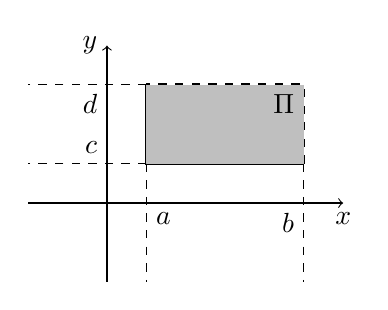
\begin{tikzpicture}[baseline={(current bounding box.north)}]
                \draw [->] (-1, 0) -- (3, 0);
                \draw [->] (0, -1) -- (0, 2);
                \draw [very thick] (0.5,1.5) -- (0.5,0.5) -- (2.5,0.5);
                \draw [dashed, very thick] (2.5,0.5) -- (2.5,1.5) -- (0.5,1.5);
                \fill [lightgray] (0.5,0.5) rectangle (2.5,1.5);
                \draw [dashed] (0.5, 0.5) -- (-1, 0.5);
                \draw [dashed] (0.5, 0.5) -- (0.5, -1);
                \draw [dashed] (0.5, 1.5) -- (-1, 1.5);
                \draw [dashed] (2.5, 0.5) -- (2.5, -1);
                \node [below right] at (0.5, 0) {$a$};
                \node [below left] at (2.5, 0) {$b$};
                \node [above left] at (0, 0.5) {$c$};
                \node [below left] at (0, 1.5) {$d$};
                \node [below] at (3, 0) {$x$};
                \node [left] at (0, 2) {$y$};
                \node [below left] at (2.5, 1.5) {$\Pi$};
            \end{tikzpicture} & 
            $D = \left\{\vec{\xi} \in \Pi\right\}$ та 
            $E = \left\{\xi_1 < b, \xi_2 < d\right\}$.
            Оскільки
            $E = A \cup B \cup C \cup D$, причому $A$, $B$, $C$, $D$ попарно несумісні, то
            $\P(E) = \P(A) + \P(B) + \P(C) + \P(D)$.
            $\P(E) = F(b, d)$, $\P(A) = F(a, c)$, $\P(B) = F(b,c) - F(a,c)$,
            $\P(C) = F(a, d) - F(a, c)$. 
            
            Отже, $\P\left\{\vec{\xi} \in \Pi\right\} = F(b,d) + F(a,c) - F(b,c) - F(a,d)$.
        \end{tabular}
    \end{proof}
\end{enumerate}

Означення сумісної функції розподілу та всі властивості узагальнюються і на випадкові вектори довільної розмірності.
\begin{definition} \index{функція розподілу!сумісна}
    \emph{Сумісною функцією розподілу} $n$-вимірного випадкового вектора $\vec{\xi}$ 
    називається $F_{\vec{\xi}}(\vec{x}) = \P\left\{\omega: \xi_1 < x_1, \xi_2 < x_2, ..., \xi_n < x_n\right\}$, $\vec{x} \in \mathbb{R}^n$.
    Функції розподілу координат цього випадкового вектора називаються \emph{маргінальними функціями розподілу} \index{функція розподілу!маргінальна}.
\end{definition}
\begin{definition}\index{випадкова величина!незалежні величини!в сукупності}
    Випадкові величини $\xi_1, \xi_2, ..., \xi_n$ називаються
    \emph{незалежними (у сукупності)}, якщо для всіх
    $x_1, x_2, ... , x_n$
    події $\left\{\xi_k < x_k\right\}, k=1,...,n$ є незалежними в сукупності.
\end{definition}

\noindent\textbf{Властивості сумісної функції розподілу:}
\begin{enumerate}
    \item Область визначення --- $\mathbb{R}^n$, область значень --- $\left<0; 1\right>$.
    \item Є монотонно неспадною за кожним аргументом.
    \item Є неперервною зліва за кожним аргументом.
    \item $\forall k = 1,...,n: \underset{x_k \to -\infty}{\lim} F_{\vec{\xi}}(\vec{x}) = 0$.
    \item $\lim\limits_{x_1, ..., x_n \rightarrow +\infty} F_{\vec{\xi}}(\vec{x}) = 1$.
    \item \emph{<<Умови узгодженості>>} \index{умова!узгодженості (умови)}: 
        $$\forall k = 1,...,n: \lim\limits_{\forall i\neq k : x_i \to + \infty} F_{\vec{\xi}}(\vec{x}) = F_{\xi_k}(x_k)$$
        $$\forall I = \left\{i_1, i_2, ..., i_k\right\} \subset \{1,...,n\}: 
        \lim\limits_{\forall i \notin I : x_i \to + \infty} F_{\vec{\xi}}(\vec{x}) =
        F_{\xi_{i_1} \xi_{i_2} ... \xi_{i_k}}(x_{i_1}, x_{i_2}, ..., x_{i_k})$$.
    \item Якщо координати $\xi_1, \xi_2, ..., \xi_n$ є незалежними у сукупності, то 
    $F_{\vec{\xi}}(\vec{x}) = F_{\xi_1}(x_1) \cdot ... \cdot F_{\xi_n}(x_n)$.
\end{enumerate}
\begin{exercise}
    Довести ці властивості.
\end{exercise}

\subsection{Дискретні випадкові вектори}
\begin{definition}\index{випадковий вектор!дискретний}
    Випадковий вектор називається \emph{дискретним}, якщо всі його координати --- 
    дискретні випадкові величини.
\end{definition}

Закон розподілу двовимірного дискретного випадкового вектора задається 
\emph{таблицею розподілу}:\index{таблиця розподілу}

\begin{center}
\begin{tabular}{c c}
    \begin{tabular}{|c|c|c|c|c|}
        \hline
        \diagbox{$\xi_2$}{$\xi_1$} & $x_1$ & $x_2$ & ... & $x_n$ \\
        \hline
        $y_1$ & $p_{11}$ & $p_{21}$ & ... & $p_{n1}$ \\
        \hline
        $y_2$ & $p_{12}$ & $p_{22}$ & ... & $p_{n2}$ \\
        \hline
        ... & ... & ... & $p_{ij}$ & ... \\
        \hline
        $y_m$ & $p_{1m}$ & $p_{2m}$ & ... & $p_{nm}$ \\
        \hline
    \end{tabular} 
    &
    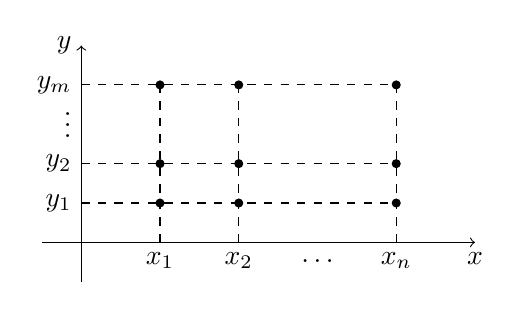
\begin{tikzpicture}[baseline={(current bounding box.center)}]
        \draw [->] (-0.5, 0) -- (5, 0); 
        \draw [->] (0, -0.5) -- (0, 2.5);
        %\draw [fill] (1, 1) circle [radius = 0.05];
        \foreach \i in {1,...,2}:
            %\draw [dashed] (\i, 0) -- (\i, 1.5);
            \foreach \j in {1,...,2}:
                \draw [fill] (\i, {\j/2}) circle [radius = 0.05];
        \foreach \k in {1,...,2} {
            \draw [fill] (4, {\k/2}) circle [radius = 0.05];
            \draw [fill] (\k, 2) circle [radius = 0.05];
            \draw [dashed] (\k, 0) -- (\k, 2);
            \node [below] at (\k, 0) {$x_\k$};
            \node [left] at (0, {\k/2}) {$y_\k$};
            \draw [dashed] (0, {\k/2}) -- (4, {\k/2});
        }
        \draw [fill] (4, 2) circle [radius = 0.05];
        \draw [dashed] (4, 0) -- (4, 2);
        \node [below] at (3, -0.1) {$\ldots$};
        \node [below] at (4, 0) {$x_n$};
        \node [below] at (5, 0) {$x$};
        \draw [dashed] (0, 2) -- (4, 2);
        \node [left] at (0, 1.6) {$\vdots$};
        \node [left] at (0, 2) {$y_m$};
        \node [left] at (0, 2.5) {$y$};
    \end{tikzpicture} \\
    $p_{ij} = \P\left\{\xi_1 = x_i, \xi_2 = y_j\right\}$, $\sum\limits_{i,j} p_{ij} = 1$ & \\
\end{tabular}
\end{center}

З таблиці розподілу можна обчислити ряди розподілу $\xi_1$ та $\xi_2$:\index{ряд розподілу}
\begin{center}
    \begin{tabular}{c c}
        \begin{tabular}{|c|c|c|c|c|}
            \hline
            $\xi_1$ & $x_1$ & $x_2$ & $...$ & $x_n$ \\
            \hline
            $p$ & $\sum\limits_{k=1}^m p_{1k}$ & $\sum\limits_{k=1}^m p_{2k}$ & $...$ & $\sum\limits_{k=1}^m p_{nk}$ \\
            \hline
        \end{tabular} &
        \begin{tabular}{|c|c|c|c|c|}
            \hline
            $\xi_2$ & $y_1$ & $y_2$ & $...$ & $y_m$ \\
            \hline
            $p$ & $\sum\limits_{k=1}^n p_{k1}$ & $\sum\limits_{k=1}^n p_{k2}$ & $...$ & $\sum\limits_{k=1}^n p_{km}$ \\
            \hline
        \end{tabular}
    \end{tabular}
\end{center}

\begin{remark}
    Обчислити таблицю розподілу, знаючи ряди розподілу координат, можна лише у випадку їх незалежності.
\end{remark}

Побудову функції розподілу для дискретного випадкового вектора простіше розглянути на прикладі.
\begin{example}
    Нехай двовимірний випадковий вектор  задано таблицею розподілу:
    \begin{center}
        \begin{tabular}{c c}
            \begin{tabular}{|c|c|c|}
                \hline
                \diagbox{$\xi_2$}{$\xi_1$} & $1$ & $2$ \\
                \hline
                $0$ & $0.3$ & $0.4$ \\
                \hline
                $1$ & $0.2$ & $0.1$ \\
                \hline
            \end{tabular}
            &
            \begin{tikzpicture}[baseline={(current bounding box.center)}]
                \draw [->] (-0.5, 0) -- (3, 0); 
                \draw [->] (0, -0.5) -- (0, 2);
                \draw [fill] (1, 0) circle [radius = 0.05];
                \draw [fill] (1, 1) circle [radius = 0.05];
                \draw [fill] (2, 0) circle [radius = 0.05];
                \draw [fill] (2, 1) circle [radius = 0.05];
                \draw [dashed] (0, 1) -- (2, 1);
                \draw [dashed] (1, 1) -- (1, 0);
                \draw [dashed] (2, 1) -- (2, 0);
                \node [below] at (1, 0) {$1$};
                \node [below] at (2, 0) {$2$};
                \node [left] at (0, 1) {$1$};
                \node [below left] at (0, 0) {$0$};
                \node [below] at (3, 0) {$t$};
                \node [left] at (0, 2) {$s$};
            \end{tikzpicture}
        \end{tabular}
    \end{center}
\end{example}
Значення функції розподілу також зручно звести в таблицю:
\begin{center}
    \begin{tabular}{|c|c|c|c|}
        \hline
        \diagbox[height=2em, width=6em]{$y$}{$x$} & $x\leq1$ & $1<x\leq2$ & $x> 2$ \\
        \hline
        $y\leq0$ & $0$ & $0$ & $0$ \\
        \hline
        $0<y\leq 1$ & $0$ & $0.3$ & $0.7$ \\
        \hline
        $y>1$ & $0$ & $0.5$ & $1$ \\
        \hline
    \end{tabular}
\end{center}
Суть побудови цієї таблиці --- у підрахунку кількості точок, що потрапляють у
квадрант $\left\{t < x, s < y \right\}$ при різних значеннях
$x$ та $y$, та обчисленні відповідних ймовірностей. Зауважимо,
що з умов узгодженості випливає, що
останній рядок таблиці --- значення $F_{\xi_1} (x)$, 
а останній стовпчик --- значення $F_{\xi_2} (y)$.